\documentclass[tikz,border=6pt]{standalone}
\usepackage{pgfplots}
\pgfplotsset{compat=1.18}
\usepgfplotslibrary{colormaps}
\usetikzlibrary{arrows, arrows.meta, calc}
\usetikzlibrary{decorations.markings}


\usepackage{amssymb,amsmath,mathtools}

\usepackage[T1]{fontenc}
\usepackage[utf8]{inputenc}
\usepackage{newpxtext,newpxmath}
\usepackage{sectsty}

\renewcommand{\Re}{\operatorname{\mathrm{Re}}}
\renewcommand{\Im}{\operatorname{\mathrm{Im}}}

\begin{document}
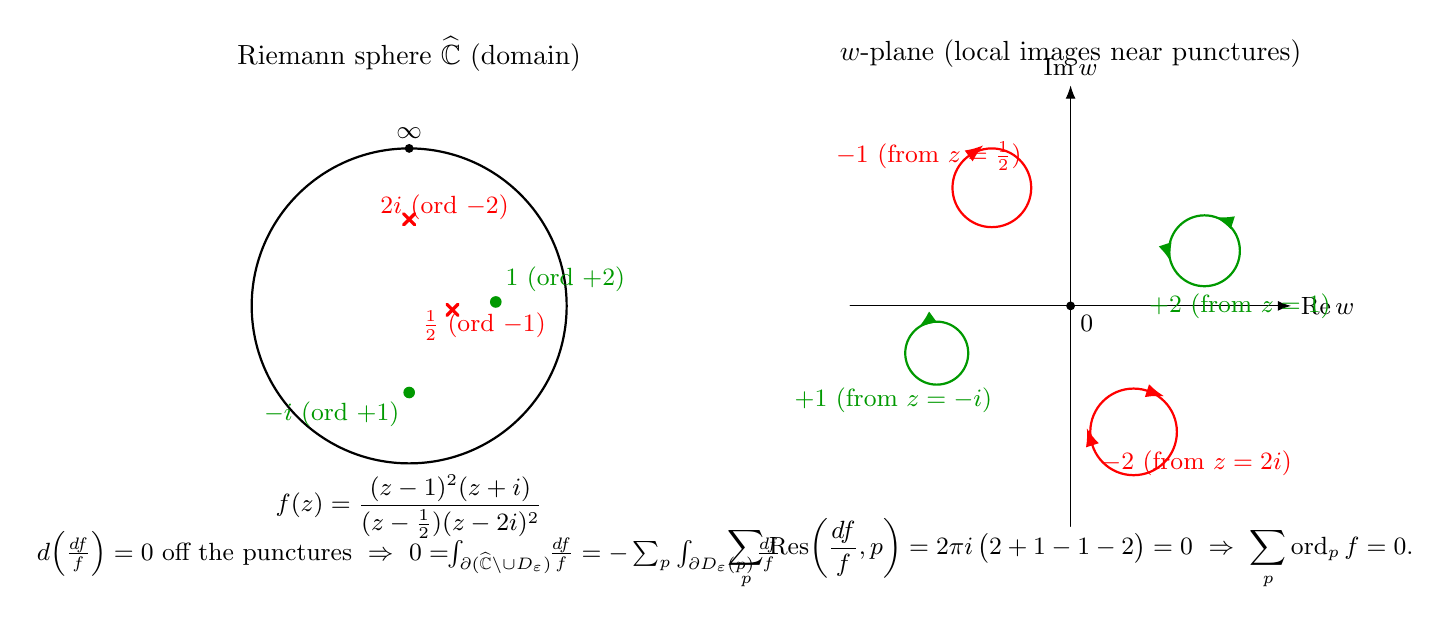
\begin{tikzpicture}[>=Latex, line cap=round, line join=round, font=\small]
	
	% ===== Left: Riemann sphere with excised disks (zeros/poles) =====
	\begin{scope}
		\node[font=\normalsize] at (0,3.2) {Riemann sphere $\widehat{\mathbb C}$ (domain)};
		% sphere silhouette
		\draw[thick] (0,0) circle (2.0);
		\fill (0,2.0) circle(1.6pt) node[above] {$\infty$};
		
		% Labels for f
		\node at (0,-2.55) {$\displaystyle f(z)=\frac{(z-1)^2(z+i)}{(z-\tfrac12)(z-2i)^2}$};
		
		% Mark zeros (green) and poles (red) roughly placed
		% zero +2 at 1
		\fill[green!60!black] (1.1,0.05) circle(2.1pt) node[above right] {$1$ (ord $+2$)};
		% zero +1 at -i
		\fill[green!60!black] (0,-1.1) circle(2.1pt) node[below left] {$-i$ (ord $+1$)};
		
		% pole -1 at 1/2
		\draw[red,very thick] (0.55,-0.05) ++(-0.07,-0.07) -- ++(0.14,0.14);
		\draw[red,very thick] (0.55,-0.05) ++(-0.07,0.07) -- ++(0.14,-0.14);
		\node[red] at (0.95, -0.25) {$\tfrac12$ (ord $-1$)};
		
		% pole -2 at 2i
		\draw[red,very thick] (0,1.1) ++(-0.07,-0.07) -- ++(0.14,0.14);
		\draw[red,very thick] (0,1.1) ++(-0.07,0.07) -- ++(0.14,-0.14);
		\node[red] at (0.45, 1.25) {$2i$ (ord $-2$)};
		
		% small inner boundaries (clockwise) around each puncture
%		\foreach \P in {(1.1,0.05),(0,-1.1),(0.55,-0.05),(0,1.1)}{
%			\draw[blue,thick,postaction={decorate},
%			decoration={markings, mark=at position 0.2 with {\arrow{<}}}] (\P) circle (0.25);
%		}
		
		% Stokes text
		\node[align=center] at (0,-3.15) {$d\!\left(\frac{df}{f}\right)=0\text{ off the punctures} \ \Rightarrow\
			0=\!\!\int_{\partial(\widehat{\mathbb C}\setminus\cup D_\varepsilon)}\!\!\frac{df}{f}
			=-\sum_{p}\int_{\partial D_\varepsilon(p)}\!\frac{df}{f}$};
	\end{scope}
	
	% ===== Right: w-plane image loops about 0 (sign = order) =====
	\begin{scope}[shift={(8.4,0)}]
		\node[font=\normalsize] at (0,3.2) {$w$-plane (local images near punctures)};
		\draw[->] (-2.8,0)--(2.8,0) node[right] {$\Re w$};
		\draw[->] (0,-2.8)--(0,2.8) node[above] {$\Im w$};
		\fill (0,0) circle (1.6pt) node[below right] {$0$};
		
		% zeros -> CCW loops, with multiplicities +2 and +1
		\draw[green!60!black,thick,postaction={decorate},
		decoration={markings,
			mark=at position 0.20 with {\arrow{>}},
			mark=at position 0.55 with {\arrow{>}}}]
		(1.7,0.7) circle (0.45);
		\node[green!60!black] at (2.15,0.0) {$+2$ (from $z=1$)};
		
		\draw[green!60!black,thick,postaction={decorate},
		decoration={markings, mark=at position 0.35 with {\arrow{>}}}]
		(-1.7,-0.6) circle (0.40);
		\node[green!60!black] at (-2.25,-1.2) {$+1$ (from $z=-i$)};
		
		% poles -> CW loops, with multiplicities -1 and -2
		\draw[red,thick,postaction={decorate},
		decoration={markings, mark=at position 0.35 with {\arrow{<}}}]
		(-1.0,1.5) circle (0.5);
		\node[red] at (-1.8,1.9) {$-1$ (from $z=\tfrac12$)};
		
		\draw[red,thick,postaction={decorate},
		decoration={markings,
			mark=at position 0.20 with {\arrow{<}},
			mark=at position 0.55 with {\arrow{<}}}]
		(0.8,-1.6) circle (0.55);
		\node[red] at (1.6,-2.0) {$-2$ (from $z=2i$)};
		
		% Sum=0 annotation (residues/ord add to zero)
		\node[align=center] at (0,-3.15)
		{$\displaystyle \sum_p \operatorname{Res}\!\left(\frac{df}{f},p\right)
			= 2\pi i\,\big(2+1-1-2\big)=0
			\ \Rightarrow\ 
			\sum_p \operatorname{ord}_p f=0.$};
	\end{scope}
	
\end{tikzpicture}
\end{document}
